% mnras_template.tex 
%
% LaTeX template for creating an MNRAS paper
%
% v3.0 released 14 May 2015
% (version numbers match those of mnras.cls)
%
% Copyright (C) Royal Astronomical Society 2015
% Authors:
% Keith T. Smith (Royal Astronomical Society)

% Change log
%
% v3.0 May 2015
%    Renamed to match the new package name
%    Version number matches mnras.cls
%    A few minor tweaks to wording
% v1.0 September 2013
%    Beta testing only - never publicly released
%    First version: a simple (ish) template for creating an MNRAS paper

%%%%%%%%%%%%%%%%%%%%%%%%%%%%%%%%%%%%%%%%%%%%%%%%%%
% Basic setup. Most papers should leave these options alone.
\documentclass[fleqn,usenatbib]{mnras}

% MNRAS is set in Times font. If you don't have this installed (most LaTeX
% installations will be fine) or prefer the old Computer Modern fonts, comment
% out the following line
\usepackage{newtxtext,newtxmath}
% Depending on your LaTeX fonts installation, you might get better results with one of these:
%\usepackage{mathptmx}
%\usepackage{txfonts}

% Use vector fonts, so it zooms properly in on-screen viewing software
% Don't change these lines unless you know what you are doing
\usepackage[T1]{fontenc}

% Allow "Thomas van Noord" and "Simon de Laguarde" and alike to be sorted by "N" and "L" etc. in the bibliography.
% Write the name in the bibliography as "\VAN{Noord}{Van}{van} Noord, Thomas"
\DeclareRobustCommand{\VAN}[3]{#2}
\let\VANthebibliography\thebibliography
\def\thebibliography{\DeclareRobustCommand{\VAN}[3]{##3}\VANthebibliography}


%%%%% AUTHORS - PLACE YOUR OWN PACKAGES HERE %%%%%

% Only include extra packages if you really need them. Common packages are:
\usepackage{graphicx}	% Including figure files
\usepackage{amsmath}	% Advanced maths commands
% \usepackage{amssymb}	% Extra maths symbols
\usepackage{siunitx}

%%%%%%%%%%%%%%%%%%%%%%%%%%%%%%%%%%%%%%%%%%%%%%%%%%

%%%%% AUTHORS - PLACE YOUR OWN COMMANDS HERE %%%%%
\DeclareSIUnit \h {\ensuremath{\mathit{h}}}
\DeclareSIUnit \parsec {pc}
% Please keep new commands to a minimum, and use \newcommand not \def to avoid
% overwriting existing commands. Example:
%\newcommand{\pcm}{\,cm$^{-2}$}	% per cm-squared

%%%%%%%%%%%%%%%%%%%%%%%%%%%%%%%%%%%%%%%%%%%%%%%%%%

%%%%%%%%%%%%%%%%%%% TITLE PAGE %%%%%%%%%%%%%%%%%%%

% Title of the paper, and the short title which is used in the headers.
% Keep the title short and informative.
\title[Cosmic Voids]{Brimming Emptiness: A Study of Formation, Evolution and Dynamics of Cosmological Voids}

% The list of authors, and the short list which is used in the headers.
% If you need two or more lines of authors, add an extra line using \newauthor
\author[Maitrey Sharma]{
Maitrey Sharma\thanks{E-mail: maitrey.sharma@niser.ac.in}
\\
% List of institutions
School of Physical Sciences, National Institute of Science Education and Research, HBNI, Jatni-752050, India\\
}

% These dates will be filled out by the publisher
%\date{Accepted XXX. Received YYY; in original form ZZZ}

% Enter the current year, for the copyright statements etc.
\pubyear{2022}

% Don't change these lines
\begin{document}
\label{firstpage}
\pagerange{\pageref{firstpage}--\pageref{lastpage}}
\maketitle

% Abstract of the paper
\begin{abstract}
Cosmological voids form the major volume of the cosmic web and therefore their influence on the evolution of Universe can provide invaluable insights into the nature of our cosmic neighborhood and beyond. We begin by developing the basic tools that help us to quantitatively define the large-scale Universe. We then present current theoretical literature on void formation, evolution and their dynamics. The void dynamics is explored by discussing elementary models of void evolution and how they are incorporated into the state-of-the-art simulations. We also touch upon how voids interact with each other, with mergers and collapses and their influence on population statistics. We sum up and tie our arguments by discussing the void galaxies and how they form an integral part of equation in study of galaxy formation and how recent observations related to them may challenge the current standard cosmological paradigms.
\end{abstract}

% Select between one and six entries from the list of approved keywords.
% Don't make up new ones.
\begin{keywords}
large-scale structure -- cosmological voids -- void galaxies
\end{keywords}

%%%%%%%%%%%%%%%%%%%%%%%%%%%%%%%%%%%%%%%%%%%%%%%%%%

%%%%%%%%%%%%%%%%% BODY OF PAPER %%%%%%%%%%%%%%%%%%

\section{Introduction}

The scale of observable universe is immense. And on these megaparsec scales, the distribution of matter is not uniform but rather forms a sprawling intricate nexus of galactic filaments, the largest known structures in the Universe, to form what is referred as the \textit{cosmic web} \citep{bond_how_1996}. Although the most prominent and defining features of the cosmic web are the filaments, it is the vast under-dense regions called cosmological voids, practically devoid of any galaxy, which occupy the most of the space in the Universe \citep{libeskind_tracing_2018, van_de_weygaert_voids_2014}. Thus, voids are integral to understanding the spatial organization and evolution of the cosmic web \citep{icke_voids_1984, sahni_evolution_1994, sheth_hierarchy_2004, einasto_wavelet_2011, aragon-calvo_hierarchical_2013}. 

\begin{figure}
	\centering
	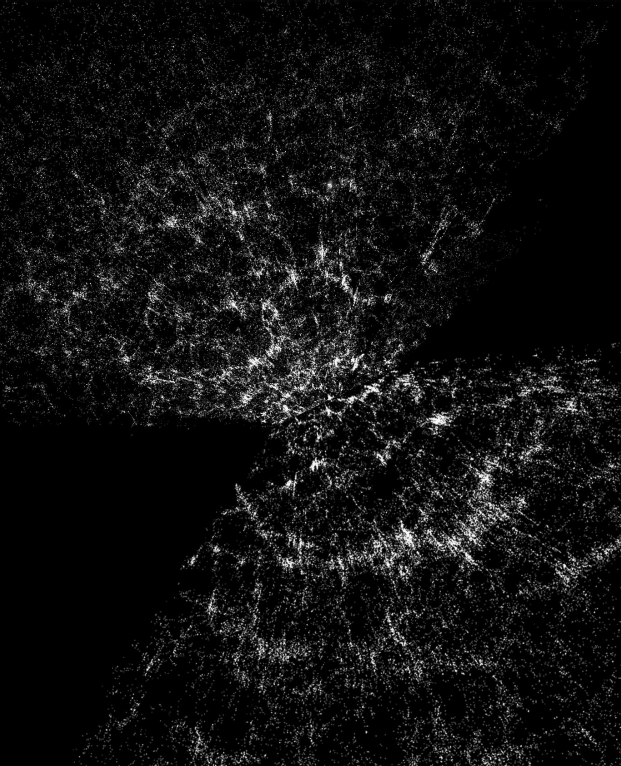
\includegraphics[scale = 0.65]{sdss_redshift}
	\caption{A still from a movie based on the data from the Sloan Digital Sky Survey (SDSS), the largest and most comprehensive sky survey till date, depicting the redshift distortion map from the third public data release of the SDSS. In these type of surveys, first data is gathered from imaging a selected specific part of sky by an observatory (for SDSS it is the Apache Point observatory in New Mexico, USA) and then doing spectroscopic analysis of the same part of sky to correlate with the laboratory values of the redshift of prominent spectral lines. Both of these types of data are combined to construct maps like above \citep{van_de_weygaert_cosmic_2011}.}
	\label{fig:sdss_rdshft}
\end{figure}


The insights aided by surveying projects like the 2dF (Two-degree field) Galaxy Redshift Survey \citep{colless_2df_2001} and the Sloan Digital Sky Survey \citep{tegmark_threedimensional_2004} building upon early galaxy redshift surveys \citep{chincarini_size_1975, gregory_perseuspisces_1978, zeldovich_giant_1982} established voids as an integral component of the cosmic web. With further developments, it has now been realized that voids not only represent an integral part of the cosmic web but also act as excellent probes and measures of global cosmology \citep{van_de_weygaert_voids_2014}.

Voids can be seen as as treasure trove of information on the cosmological environment and related parameters. The outflowing mass and accompanying redshift distortion maps leave a cosmological footprint which then can be analyzed to develop and improve our understanding of cosmology as whole \citep{martel_simulation_1990, dekel_omega_1994, ryden_voids_1996}. The undisturbed and untainted low-density environments of voids represents an ideal and pure setting for the study of galaxy formation and the influence of cosmic environment on the formation of galaxies \citep{kreckel_only_2011, kreckel_void_2012}. Furthermore, voids have also been believed to have played a prominent role in the reionization process in the early Universe \citep{furlanetto_cosmology_2006, morales_reionization_2010}.

In this review of these crucial features of the cosmic web, we will start with building the foundations of cosmology and will explore how large-scale structures of the Universe can be quantitatively described. After that, we will build upon the existing reviews \citep{van_de_weygaert_cosmic_2011, van_de_weygaert_voids_2014} to understand the formation, evolution and dynamics of voids and will comment on their current state of research by discussing theoretical models and how they complement to observations. We will also explore the void galaxies, the lonesome galaxies located in the voids, as they provide key constraints on our understanding of galaxy formation in a cosmological context \citep{kreckel_void_2014}. We will also discuss the discourses the study of cosmic voids has transpired in broader domains of cosmology relating to dark energy and the standard cosmological model. In the end, after contemplating the results, we will discuss the future of the research in this field.
%This is a simple template for authors to write new MNRAS papers.
%See \texttt{mnras\_sample.tex} for a more complex example, and \texttt{mnras\_guide.tex}
%for a full user guide.
%
%All papers should start with an Introduction section, which sets the work
%in context, cites relevant earlier studies in the field by \citet{Fournier1901},
%and describes the problem the authors aim to solve \citep[e.g.][]{vanDijk1902}.
%Multiple citations can be joined in a simple way like \citet{deLaguarde1903, delaGuarde1904}.

\section{The Large-scale Universe}
In order to formally study large-scale structures of the Universe like cosmological voids, it is essential to be well-versed through fundamentals of physical cosmology. In this section, we will lay the foundations that trace their origins all the way back to Einstein's theory of general relativity and will develop techniques that enable us to quantitatively describe the large-scale Universe. 
%Normally the next section describes the techniques the authors used.
%It is frequently split into subsections, such as Section~\ref{sec:maths} below.

\subsection{The Friedmann Equations}
In 1922, using Einstein's field equations of gravitation for the Friedmann–Lema\^{i}tre–Robertson–Walker metric and a perfect fluid with a given mass density $ \rho $ and pressure $ p $, Alexander Friedmann derived his equations that govern the expansion of space in homogeneous and isotropic models of the universe \citep{friedman_uber_1922}. They are as follows:
\begin{equation}\label{key}
	\dfrac{\dot{a} + kc^2}{a^2} = \dfrac{8 \pi G \rho + \Lambda c^2}{3}
\end{equation}
and
\begin{equation}\label{key}
	\dfrac{\ddot{a}}{a} = -\dfrac{4 \pi G}{3} \Bigg(\rho + \dfrac{3p}{c^2}\Bigg) + \dfrac{\Lambda c^2}{3}
\end{equation}
\label{sec:maths} % used for referring to this section from elsewhere

Here $ a $ is a dimensionless quantity called the scale factor and it is a function of time. The scale factor acts as a parameter which describes the relative expansion rate of the Universe. $ \dot{a} $ and $ \ddot{a} $ are with respect to time. $ k $ is a constant for a particular solution, $ G $ is the Newton's gravitational constant and $ \Lambda $ is the cosmological constant.

These equations lie at the core of every theoretical model in physical cosmology and the evolution of large-scale structures like filaments and voids is described most accurately by them.

\subsection{Distance Measures}
As the Universe is expanding with time, we need a framework to specify the distances between any two points in space at any point in time. This is important when it comes to analytically study large-scale structures of the Universe. The most well-known consequence of expansion of space is the cosmological redshift, defined as the fractional Doppler shift of its emitted light resulting from radial motion \citep{hogg_distance_2000}:
\begin{equation}\label{key}
	z \equiv \dfrac{\nu_e}{\nu_o} - 1 = \dfrac{\lambda_o}{\lambda_e} - 1
\end{equation}
where $ \nu $ is the frequency, $ \lambda $ is the wavelength and subscripts $ e $ and $ o $ denote emitted and observed quantities respectively, 
\textit{Hubble's law} is the observation that all sufficiently distant objects from Earth are moving away from it at speeds proportional to their distances.

There are many ways in which distances in cosmology are defined and they all are asymptotic to each other for small redshifts. Further, it is actually convenient to express these distances as functions of redshift since it is always an observable.

The \textit{comoving distance} is one of the most important distance type and can be contrasted with \textit{proper distance} as the distance which remains constant over cosmological time as it takes account for the expansion of the Universe. It is defined as:
\begin{equation}\label{key}
	d_C (z) = d_H \int_0^z \dfrac{dz'}{E(z')}
\end{equation}
along the line of sight (LOS), where $ d_H $ is the \textit{Hubble distance}, given by $ d_H = c/H_0 \approx \SI{3000}{\per \h \mega \parsec} = \SI{9.26e25}{\per \h \meter} $, $ c $ being speed of light and $ H_0 $ is \textit{Hubble parameter} at the present. The symbol $ h $ is the \textit{dimensionless Hubble constant} and considered a unit itself. The Hubble constant is provides the mathematical form of the Hubble's law as $ H_0 = v/D $ where $ v $ is the velocity of separation and $ D $ is cosmological time-dependent proper distance. Further, we define the \textit{dimensionless Hubble parameter} \citep{peebles_principles_1993}:
\begin{equation}\label{key}
	E (z) = \dfrac{H(z)}{H_0} = \sqrt{\Omega_r (1+z)^4 + \Omega_m (1+z)^3 + \Omega_k(1+z)^2 + \Omega_{\Lambda}}
\end{equation}
Here, $ \Omega_{r} $, $ \Omega_{m} $ and $ \Omega_{\Lambda} $ are normalized values of the present radiation energy density, matter density, and \textit{dark energy density,} respectively with $ \Omega_k = 1 - \Omega_{r} - \Omega_{m} - \Omega_{\Lambda}$ determining the curvature. 

In due course, we will see that catalogs courtesy of sky surveying projects like the \textit{Sloan Digital Sky Survey} (SDSS) often report distances related to large scale-structures like voids in form of comoving distance so it is necessary to understand this development. The Friedmann equations and different distances forms the theoretical aspect of cataloging any large-scale structure in the Universe, with observations gathered from the sky surveying projects using ground based telescopes and even in space probes (like with the \textit{Planck} project for detecting cosmic microwave background anisotropies).


\section{Formation, Evolution and Dynamics of Voids}
Moments after the Big Bang, the early Universe expanded rapidly, in the period which is known as the inflationary epoch. During this cosmic inflation, the scale factor grew exponentially, causing the quantum fluctuations, that is, temporary random changes in amount of energy at a point in space, to stretch to macroscopic scales. These manifested as variations in density and is now believed to have seeded all the structure in the Universe \citep{hartle_gravity_2003}, including the cosmological voids.

Voids represent underdensities in the Universe and consequently they produce an effectively repulsive gravitational influence. Mass flows out of the underdesnity, reducing the density as the cosmic web evolves \citep{cautun_evolution_2014}. With time, the mass distribution inside the void becomes increasingly uniform as more mass moves outwards around the boundary. Consequently, the density in these underdense regions increases as we move outward with inner regions becoming more and more becoming like low-density FRW Universe \citep{goldberg_simulating_2004}. This mechanism prevents formation of any prominent substructure \citep{cautun_evolution_2014}.

Except for a few like \citet{icke_voids_1984}, most of the early theoretical models of void formation were concerned with evolution of isolated voids \citep{hoffman_origin_1982, bertschinger_self-similar_1985, blumenthal_largest_1992} with spherically symmetric configurations, but in reality, as voids evolve and expand in size and inevitably are influenced by their also expanding peers. Though still, they can provide a lot of information. 

\subsection{Spherical void evolution}
As a differential develops in density layers from inner regions to outwards regions. The greater mass in outward regions experiences more moderate interior underdensity and thus inner layers move faster than the outward layers. Eventually, the interior mass shells take over the exterior shells, and this process is referred as \textit{shellcrossing}.

The spherical void evolution can be studied in two regimes: linear and non-linear. For a density field $ \rho (\textbf{x}, t) $ at comoving coordinate $ x $ and time $ t $ with a mean of $ \bar{\rho}(t) $. The desnity contrast is defined as
\begin{equation}\label{key}
	\delta (\textbf{x}, t) = \dfrac{\rho (\textbf{x}, t)}{\bar{\rho}(t)} -1
\end{equation}
After applying conservation of mass we can factorize  it into time-dependent and space-dependent factors using a linear growth factor $ D(t) $,
\begin{equation}\label{key}
	\delta (\textbf{x}, t) = D(t) \delta (\textbf{x})
\end{equation}
From here, after doing some mathematics of using divergence theorem and incorporating the Hubble's law, we can obtain the relation between the radial velcoity field and the average density contrast within the spherical void \citep{peebles_large-scale_1980},
\begin{equation}\label{key}
	v(r, t) =-\dfrac{1}{3} f(t) H(t) r \Delta (r, t)
\end{equation}
where $ H(t) \equiv \dot{a} (t)/a(t) $ is the Hubble flow rate, $ f(t) \equiv d \ln D(t)/d \ln a(t) $ and $ \Delta  (r, t)$ is the average density contrast within radius $ r $ as 
\begin{equation}\label{key}
	\Delta (r, t) \equiv \dfrac{3}{4 \pi r^3} \int_{V_S} \delta (\textbf{x}, t) d^3x
\end{equation}
with $ V_S $ representing the total spherical volume, $ V = (4/3) \pi r^3 $.

The non-linear regime emerges after the implementation of general relativity. After a bit of involved and not-so-trivial mathematics, we obtain the density contrast inside the \textit{tophat} or the \textit{bucket} region, which actually acts as density threshold, as $ \delta_v = \equiv -2.717 $ \citep{hamaus_universitats-sternwarte_2017}, which is intriguingly and seemingly implausible negative physical density. But as we will see, it appears prominently in the excursion set theory of void evolution.

We can relate linear and non-linear underdensities approximately by
\begin{equation}\label{key}
	\delta_v = C [1-(1+\delta_{0,sc})^{-1/C}]
\end{equation}
with $ C \simeq 1.594 $ (\citep{bernardeau_nonlinear_1994}). Void observations are done using \textit{tracers}, which are often galaxies. There have been improvements (see \cite{pollina_linearity_2017, ronconi_cosmological_2017}) in eradicating tracer bias and to get constraints on void formation using tracer density distribution.



\begin{figure}
	\centering
	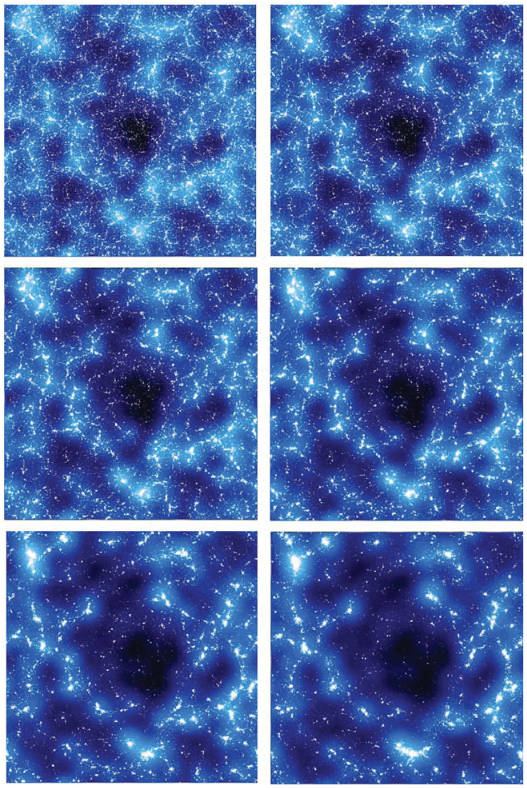
\includegraphics[scale = 0.6]{void_evol}
	\caption{Evolution of a void in the $ \Lambda$CDM scenario according to a simulation based on matter outflow in an Einstein-de Sitter Universe which incorporated the Hubble law. One can clearly see the presence of rich substructure as void evolves. Image courtesy of Erwin Platen.}
	\label{fig:voidevol}
\end{figure}
\begin{figure}
	\centering
	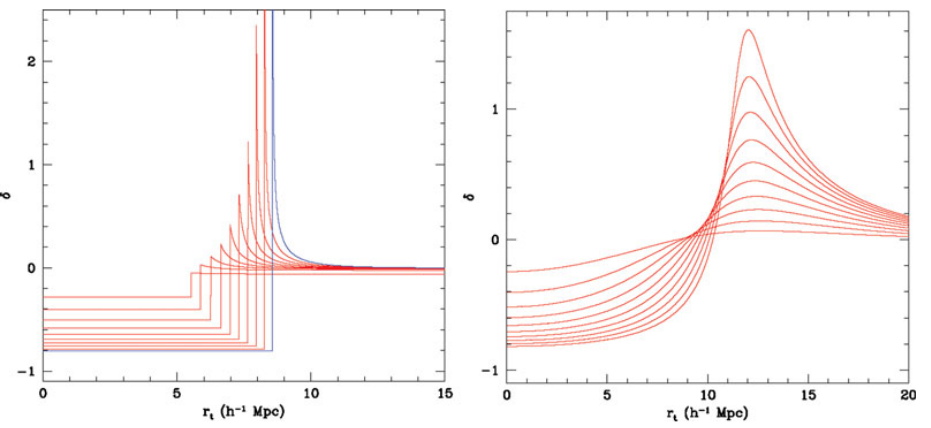
\includegraphics[scale = 0.35]{tophat}
	\caption{These plots represent what is called as the tophat or the bucket model of void evolution, due to the configuration. On left is the tophat which evolved up to the onset of shellcrossing and on the right is with treatment of the $ \Lambda$CDM model \citep{van_de_weygaert_voids_2014}.}
	\label{fig:tophat}
\end{figure}

\subsection{Void Dynamics}
Voids are not static structures as we have seen. Outflow of matter in the void leads to its expansion and it has been observed in various galaxy surveys and surveys of galaxy peculiar motions. For example, Figure \ref{fig:voidflow} presents a map of velocity flows found using the PSCz galaxy redshift survey and the effect of the Sculptor void is very apparent. Void influence is also observed individual galaxies exhibiting peculiar motion \citep{tully_our_2008}.
\begin{figure}
	\centering
	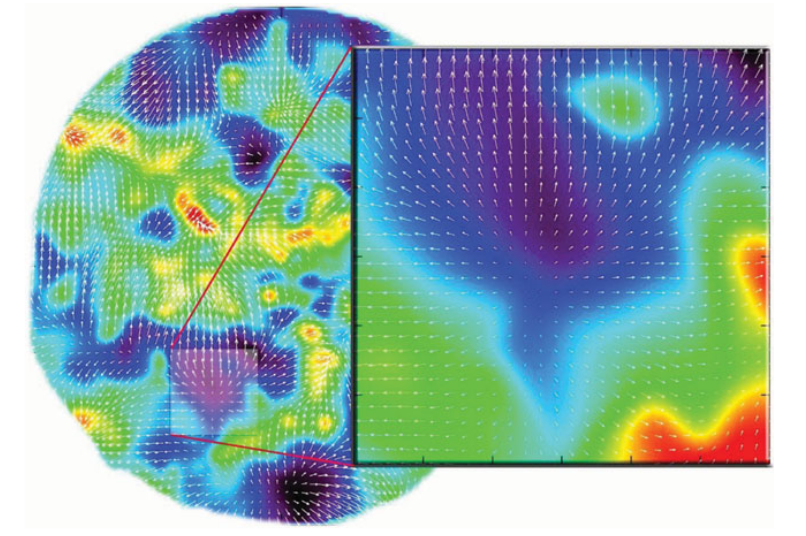
\includegraphics[scale = 0.35]{voidflow}
	\caption{The velocity outflows of matter are clearly visible from this velocity map courtesy of the PSCz survey around the Sculptor void \citep{romano-diaz_delaunay_2007}.}
	\label{fig:voidflow}
\end{figure}
Void dynamics can a number of progenitors, like tidal forces, which mainly depend on the inhomogeneous composition of the environment of voids. \cite{icke_voids_1984} propounded the idea of studying this influence using what now is called as the \textit{homogeneous ellipsoidal model} and was later expanded by \cite{white_growth_1979}, \cite{eisenstein_analytical_1995}, \cite{bond_peak-patch_1996} and \cite{desjacques_environmental_2008}.
\subsubsection{Homogeneous Ellipsoidal Model}
The homogeneous ellipsoidal model assumes an object to be a region with a triaxially symmetric ellipsoidal geometry and a homogeneous interior density, embedded within a uniform background density $ \rho_u $ . If the simple situation of the external tidal shear directed is along the principal axes of the ellipsoid then the gravitational acceleration along the principal axes of an ellipsoid with over/underdensity $ \delta $ can be evaluated from the expression for the corresponding scale factors $ \mathcal{R}_\textrm{i} $.

\begin{equation}\label{eq:hev}
	\dfrac{d^2 \mathcal{R}_\textrm{m}}{dt^2} = -4 \pi G \rho_u (t) \Bigg[\dfrac{1+\delta}{3} + \dfrac{1}{2}\Bigg(\alpha_m - \dfrac{2}{3} \Bigg)\delta \Bigg] \mathcal{R}_\textrm{m} - \tau_\textrm{m} \mathcal{R}_\textrm{m} + \Lambda \mathcal{R}_\textrm{m}
\end{equation}
Here, $ \alpha_m $ relates to the ellipsoidal geometry and is given by
\begin{equation}\label{key}
	\alpha_m (t) = \mathcal{R}_1 (t) \mathcal{R}_2 (t) \mathcal{R}_3 (t) \int_0^{\infty} \dfrac{d \lambda}{(\mathcal{R}_\textrm{m}^2 (t)+\lambda) \prod_{n=1}^{3} (\mathcal{R}_\textrm{n}^2 (t)+\lambda)^{1/2}}
\end{equation}
$ \tau_\textrm{m} $ is the eigenvalue of the tidal shear tensor $ T_{mn} $ and $ \Lambda $ is the cosmological constant. From equation \ref{eq:hev}, it is clear that $ \delta $ increases strongly in the non-linear regime and the influence of the tidal field will recede.

\subsubsection{Void Shapes}
Voids are quite non-spherical, and according to \cite{platen_alignment_2008}, they are slightly prolate with axis ratios of the order $ c : b : a \approx 0.5 : 0.7 : 1 $.  These values are verified by \cite{shandarin_shapes_2006} and \cite{park_void_2007}. 

This prolateness of voids forms the foundation of void finding algorithms. These can mainly be classified into three categories: ones that use the local galaxy density to identify voids \citep{hoyle_voids_2002}, ones that use the topology of dark matter suggested by galaxies \citep{colberg_voids_2005}, and the ones that dynamically identify voids by using gravitational unstable points in the dark matter \citep{hahn_properties_2007}. In the following paragraph, few algorithms are discussed to provide the picture how the observed data from sky surveying projects is analyzed using theoretical models to define voids. All algorithms have their own unique spin of the identification process so there is a factor of openness in how to approach this process.

Developed by \cite{el-ad_voids_1997}, the \textit{VoidFinder} algorithm takes galaxy catalogs (such as \cite{pan_cosmic_2012}) and then uses the Nearest Neighbor Approximation to calculate the cosmic density in the region contained in a spherical radius determined by the distance to the third-closest galaxy. There is the Zone Bordering on Voidness (ZOBOV) algorithm which used the Voronoi tessellation technique\footnote{Voronoi tessellation or Voronoi diagram is the partitioning of a plane with $ n $ points into convex polygons such that each polygon contains exactly one generating point and every point in a given polygon is closer to its generating point than to any other.} and mock border particles in order to categorize regions based on a high-density contrasting border with a very low amount of bias \citep{neyrinck_zobov_2008}. The Dynamical void analysis (DIVA) algorithm \citep{lavaux_precision_2010} redefines voids: instead of an underdensity, DIVA defines void as regions where matter is outflowing, echoing our theoretical description of void evolution. Introduced by \cite{platen_cosmic_2007}, the Watershed Void Finder (WVF) identifies voids via a watershed transform\footnote{Defined on a grayscale image where it treats brightness of each point as its height, much like a topographic map} applied to the DTFE (Delaunay Tessellation Field Estimator\footnote{A mathematical tool for reconstructing a volume-covering and continuous density or intensity field from a discrete point set. Delauney Tessellation or Delauney Triangulation is a connection scheme based on triplets of points (in two dimensions). Three points ($ i $, $ j $, and $ k $) are connected as a triangle if the circle which circumscribes them does not contain any other point $ l $ within its circumference.}) density field reconstruction \citep{schaap_continuous_2000, van_de_weygaert_cosmic_2009}. The wastershed transformation has close relation to the topology of the cosmic web \citep{aragon-calvo_spine_2010} and therefore the WVF algorithm has attracted a decent amount of attention \citep{colberg_aspenamsterdam_2008, neyrinck_zobov_2008, sutter_observability_2015, nadathur_nature_2015}.

The influx of new and improved from surveys like 2MASS redshift survey have enhanced our understanding of the dyanmics of cosmic web, with the role of voids being most convincingly demonstrated by the Cosmicflows2, Cosmicflows3 and Cosmicflows4 projects \citep{tully_our_2008, courtois_three-dimensional_2012, kourkchi_cosmicflows-4_2020, kourkchi_cosmicflows-4_2022}.
\subsection{Void Sociology}
Advancements in computational horsepower have enabled $ N $-body simulations which can be used to resolve substructures within voids and they have revealed rich complex scenarios, in contrast with idealised spherical or ellipsoidal models \citep{mathis_voids_2002, gottlober_structure_2003, goldberg_simulating_2004, colberg_voids_2005, padilla_spatial_2005, ceccarelli_voids_2006, bos_darkness_2012, aragon-calvo_hierarchical_2013, sutter_observability_2015, wojtak_voids_2016}. 

Void evolution is dictated by two processes: mergers and collapses. An analogy with soapsuds is made when studying the hierarchical population distribution of voids. The earliest voids, emerged from the primordial fluctuations which coexist within a large underdense region eventually merge into a larger void whereas those who are present in relatively overdense regions are pushed and squeezed out existence. When dealing with void populations, engulfed subvoids are often skipped and only the largest void is concerned. Further, recent studies have identified existence of collapsed void regions \citep{paz_clues_2013}. 
\begin{figure}
	\centering
	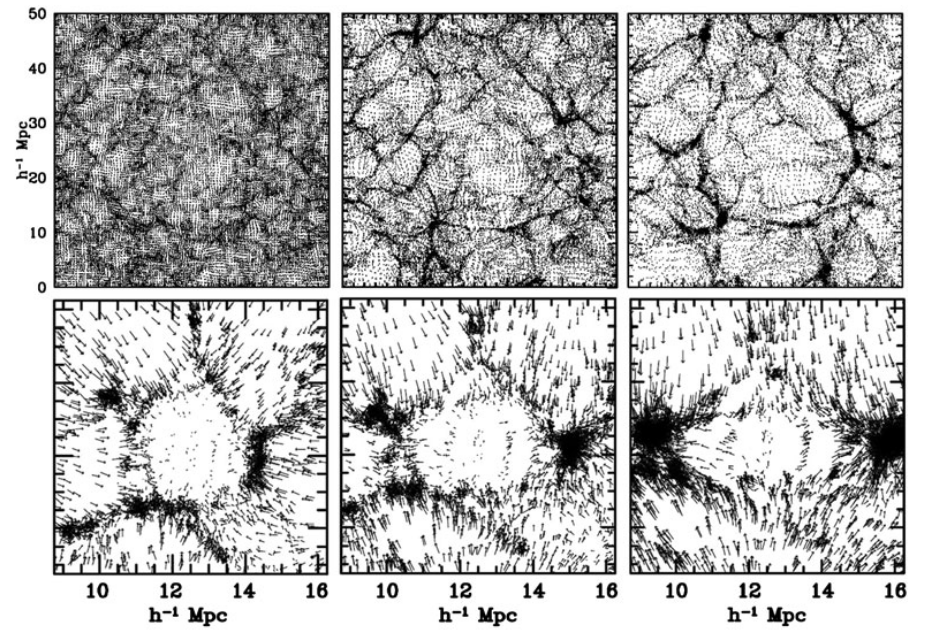
\includegraphics[scale=0.35]{mergecollapse}
	\caption{These images are obtained from the $ N $-body simulations considering a $ \Lambda $CDM Universe with the top row depecting mergers and bottom row collapses, with arrows representing velocity outflows of matter. The collapse is caused due to delta in tidal strength at the void boundaries.}
	\label{fig:mergecollapse}
\end{figure}

The void excursion theory incorporates the processes of mergers and collapse and models void populations using a two-barrier excursion set formalism \citep{sheth_hierarchy_2004}. In the extended Press-Schechter approach, using this formalism, we can predict a distribution function $ n_v (M) $ for voids on mass scale $ M $.

Ultimately, while this model provides a good framework for modelling void population, a lot of improvements can be desired from modifying large-scale environment to treatment as a prolate. One of the major issue while modelling populations is the value of the density barrier, which if derived considering spherical evolution, demands scrutiny. Some improvements have been put forward like \cite{paranjape_hierarchy_2012}, \cite{jennings_abundance_2013} and \cite{pontzen_inverted_2016}. Further, as already discussed, galaxies prove to be biased tracers at the end of the day so we end up with a myopic and limited information of void populations.


\section{Void Galaxies}
The galaxies evolving in the voids prove to be crucial when exploring galaxy evolution. They are far from any major gravitational influence and evolve in a pristine environment. And consequently many recent studies on void galaxies have appeared in the community.


With very few disturbances due to desolate neighborhood, void galaxies have distinctly different properties when compared to their counterparts residing in overdense regions. They appear to be relatively recently formed as evident by the rate of star formation in them and lack of external gravitational influence leads to less erratic gas distribution throughout.
Obervations made using sky surveying projects SDSS and 2dFGRS indicate that void galaxies lie of the bluer side of the spectrum possessing high star formation rates.

There has been few debates over some discrepancies in theoretical propositions and observations related to void galaxies. For objects with lower luminosity, discrepancies in density distribution have been reported \citep{karachentsev_catalog_2004}. Apparently, there is less than expected number of galaxies with low luminosity, that is, dwarf galaxies. This is concerning because elementary models of galaxy formation \citep{little_cosmic_1994} have predicted the opposite \citep{wyse_formation_1992}. In fact, \cite{peebles_void_2001} dared to say that these observations could challenge the current standard cosmological model itself. This is not a trivial proposition. 

Recently, \cite{tavasoli_void_2021} studied a distribution of galaxies no brighter than limiting magnitude $ M_r < -18 $ in voids using the 16th release of SDSS data and the Millennium simulation which is an $ N $-body simulation project to provide insights in the distribution and evolution of matter in the Universe and also reveal information about current galaxy populations. After defining two parameters of mean-distance and center-distance (mean-distance of all galaxies from host void center) to assign positions to the galaxies. The comparison of simulation and observed results is shown in Figure \ref{fig:tav1}. It can be inferred from this figure that on increasing void size in the simulation sample, galaxies become more far spaced out from the void center, however observations tell otherwise. The discrepencies extend to the study of density profiles (see Figure \ref{fig:tav2}). Again the same trend is observed, void size becomes a factor in the simulation whereas the observations do not seem to back that up. Of course, if these deviations are significant enough, is debatable. 

\begin{figure}
	\centering
	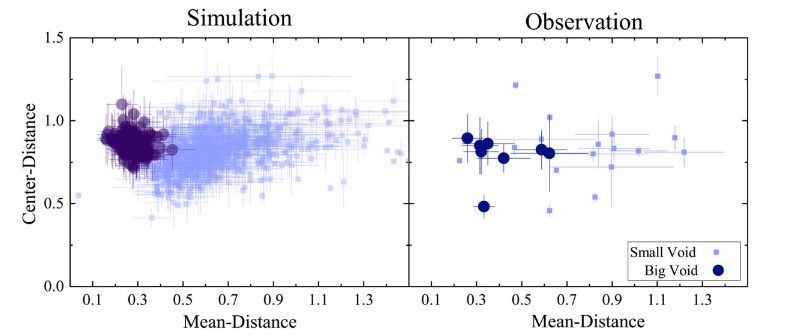
\includegraphics[scale = 0.4]{tav1}
	\caption{Spatial distribution of galaxies in a void parameterized by the mean-distance and center-distance}
	\label{fig:tav1}
\end{figure}
\begin{figure}
	\centering
	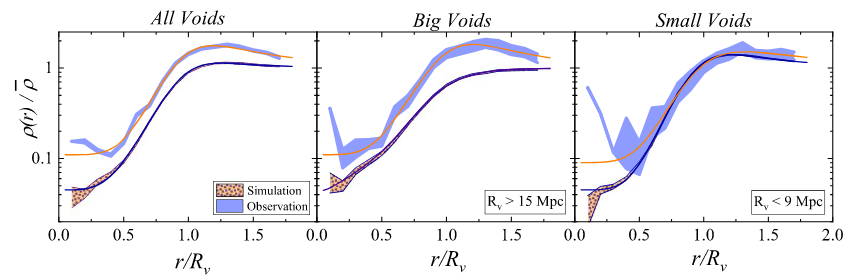
\includegraphics[scale = 0.35]{tav2}
	\caption{Stacked void density profiles again show similar trend where void size becomes a deciding factor in the simulations when having none effect in observed data}
	\label{fig:tav2}
\end{figure}


Further, our own Milky Way galaxy is believed to be a void galaxy, residing in the KBC void \citep{keenan_evidence_2013, abdalla_cosmology_2022}, and one can argue that if that makes all our generalization of our galactic neighborhood biased. Even the existence of the unusually large KBC void is debated under the $ \Lambda $CDM model \citep{haslbauer_kbc_2020}.


\section{Results}
Observational results to study any phenomena or objects in physical cosmology are delivered by the sky surveying projects. The SDSS has proved to be a landmark project in such a space. In coming years we will be witnessing influx of more improved and rich data from surveys like the Legacy Survey of Space and Time (LSST) by the Vera C. Rubin observatory which is under construction in Chile and the \textit{Euclid}, a space-bound mission which will operate in the near-infrared to map redshifts to galaxies, to be launched by the European Space Agency sometime next year. With the advancements in computational resources, new simulation models are developing which aid in extending and testing the theoretical limits of the field. Apart from the Millenium simulation, \textit{Illustris} is one such example.


\section{Conclusions}
Our aim was to fill the dearth of a robust and up-to-date review on cosmological voids motivated by the very elusive nature of the field. We explored the basics of general relativity and laid down the foundations to properly quantify distances in the large-scale Universe.  We studied void formation and evolution theoretically and saw their implementations in simulations when exploring void dynamics. We further discussed how voids interact, with smaller voids being merged to form larger voids or tidal forces leading to void collapses and how this mechanism influences void population statistics. We then finally looked at void galaxies and understood why they are so important, while noting down recent discrepancies between simulations and observations. 

Cosmological voids present a very elusive area of study in the near future with coming of the next generation of telescopes and space probes, along with advanced computer simulations. There is yet lot to be learnt about nature of dark energy and dark matter and studying of voids is bound to play a very important role in answering physical cosmology's biggest questions. All in all, the future of this field looks promising.
\section*{Acknowledgements}

I acknowledge the immensely crucial discussions with Dr. Tuhin Ghosh over the summer earlier which served as the motivation to write this review. I also thank Dr. Luke Chamandy for their the invaluable suggestions and comments to make this review as polished as possible. 

%%%%%%%%%%%%%%%%%%%%%%%%%%%%%%%%%%%%%%%%%%%%%%%%%%
%\section*{Data Availability}
%
% 
%The inclusion of a Data Availability Statement is a requirement for articles published in MNRAS. Data Availability Statements provide a standardised format for readers to understand the availability of data underlying the research results described in the article. The statement may refer to original data generated in the course of the study or to third-party data analysed in the article. The statement should describe and provide means of access, where possible, by linking to the data or providing the required accession numbers for the relevant databases or DOIs.




%%%%%%%%%%%%%%%%%%%% REFERENCES %%%%%%%%%%%%%%%%%%

% The best way to enter references is to use BibTeX:
\bibliographystyle{mnras}
\bibliography{p463} % if your bibtex file is called example.bib


% Alternatively you could enter them by hand, like this:
% This method is tedious and prone to error if you have lots of references
%\begin{thebibliography}{99}
%\bibitem[\protect\citeauthoryear{Author}{2012}]{Author2012}
%Author A.~N., 2013, Journal of Improbable Astronomy, 1, 1
%\bibitem[\protect\citeauthoryear{Others}{2013}]{Others2013}
%Others S., 2012, Journal of Interesting Stuff, 17, 198
%\end{thebibliography}

%%%%%%%%%%%%%%%%%%%%%%%%%%%%%%%%%%%%%%%%%%%%%%%%%%

%%%%%%%%%%%%%%%%% APPENDICES %%%%%%%%%%%%%%%%%%%%%





%%%%%%%%%%%%%%%%%%%%%%%%%%%%%%%%%%%%%%%%%%%%%%%%%%


% Don't change these lines
%\bsp	% typesetting comment
\label{lastpage}
\end{document}

% End of mnras_template.tex
